\documentclass[10pt]{article}
\usepackage[a4paper,margin=2cm]{geometry}
\usepackage[brazilian]{babel}
\usepackage[utf8]{inputenc}
\usepackage[T1]{fontenc}
\linespread{1.3}
\parskip=12pt
\parindent=0pt
\usepackage{enumerate}
\usepackage{amsfonts}
\usepackage{amsmath}
\usepackage{amsfonts}
\usepackage{graphicx}
\usepackage[section]{placeins}

\begin{document}
	\begin{center}
		{\Large{\textbf{Lista 1 - Métodos Numéricos}}}\\
		\vspace{0.2cm}
		EPGE/FGV - 2018\\
		Professor: Cezar Santos\\
		Aluno: Raul Guarini
	\end{center}

\section*{Calibração Original: $\rho = 0.95$}

Os códigos principais que resolvem esta lista são \texttt{ps1.m} e \texttt{ps1.py}. O primeiro passo foi construir as matrizes de transição dos processos discretizados, seguindo a calibração indicada. O parâmetro de \textit{scaling} $m$ do método de Tauchen foi calibrado como $m = 3$, seguindo os slides da aula. Encontrei as seguintes matrizes:
\begin{figure*}[h!]
	\centering
	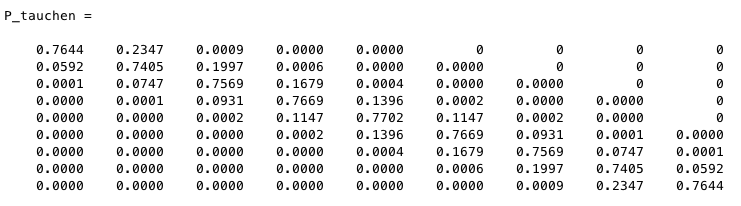
\includegraphics[scale = 0.6]{P_tauchen.png}
	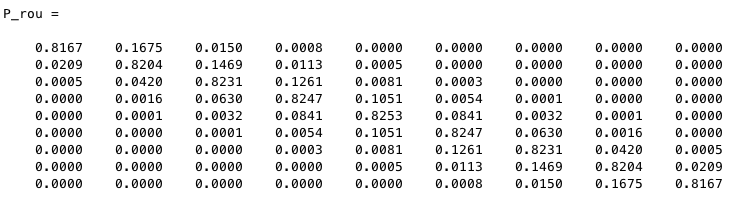
\includegraphics[scale=0.6]{P_row}
	\caption{Matrizes de Transição, $N = 9$ e $\rho = 0.95$}
\end{figure*}

Em seguida, simulei o AR(1) verdadeiro em questão por 10100 períodos, sendo os 100 primeiros períodos utilizados como ``burn'' para eliminar o efeito da condição inicial (sempre o centro do grid). O caminho simulado é ilustrado a seguir. Utilizando a mesma sequência de choques gaussianos $\epsilon_{t}$, computei os caminhos gerados pelos dois processos (Tauchen em vermelho e Rouwenhorst em verde).

\begin{figure*}[h!]
	\centering
	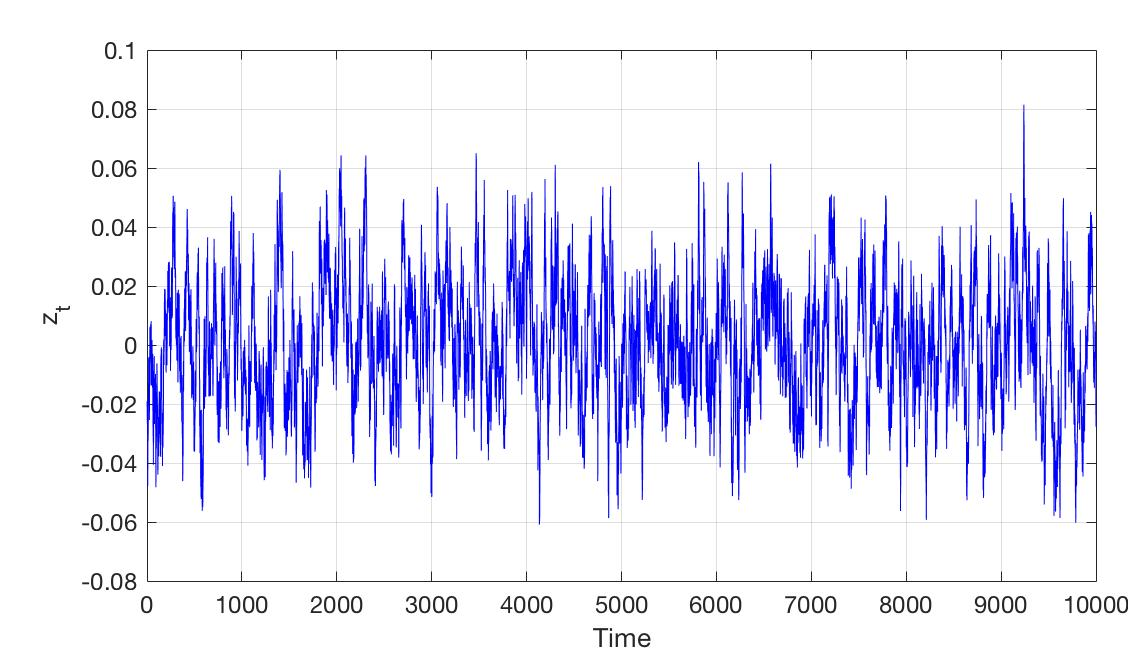
\includegraphics[scale=0.3]{cont_path.jpg}
	\caption[h!]{AR(1) Contínuo, $\rho = 0.95$}
\end{figure*}

\begin{figure*}[h!]
	\centering
	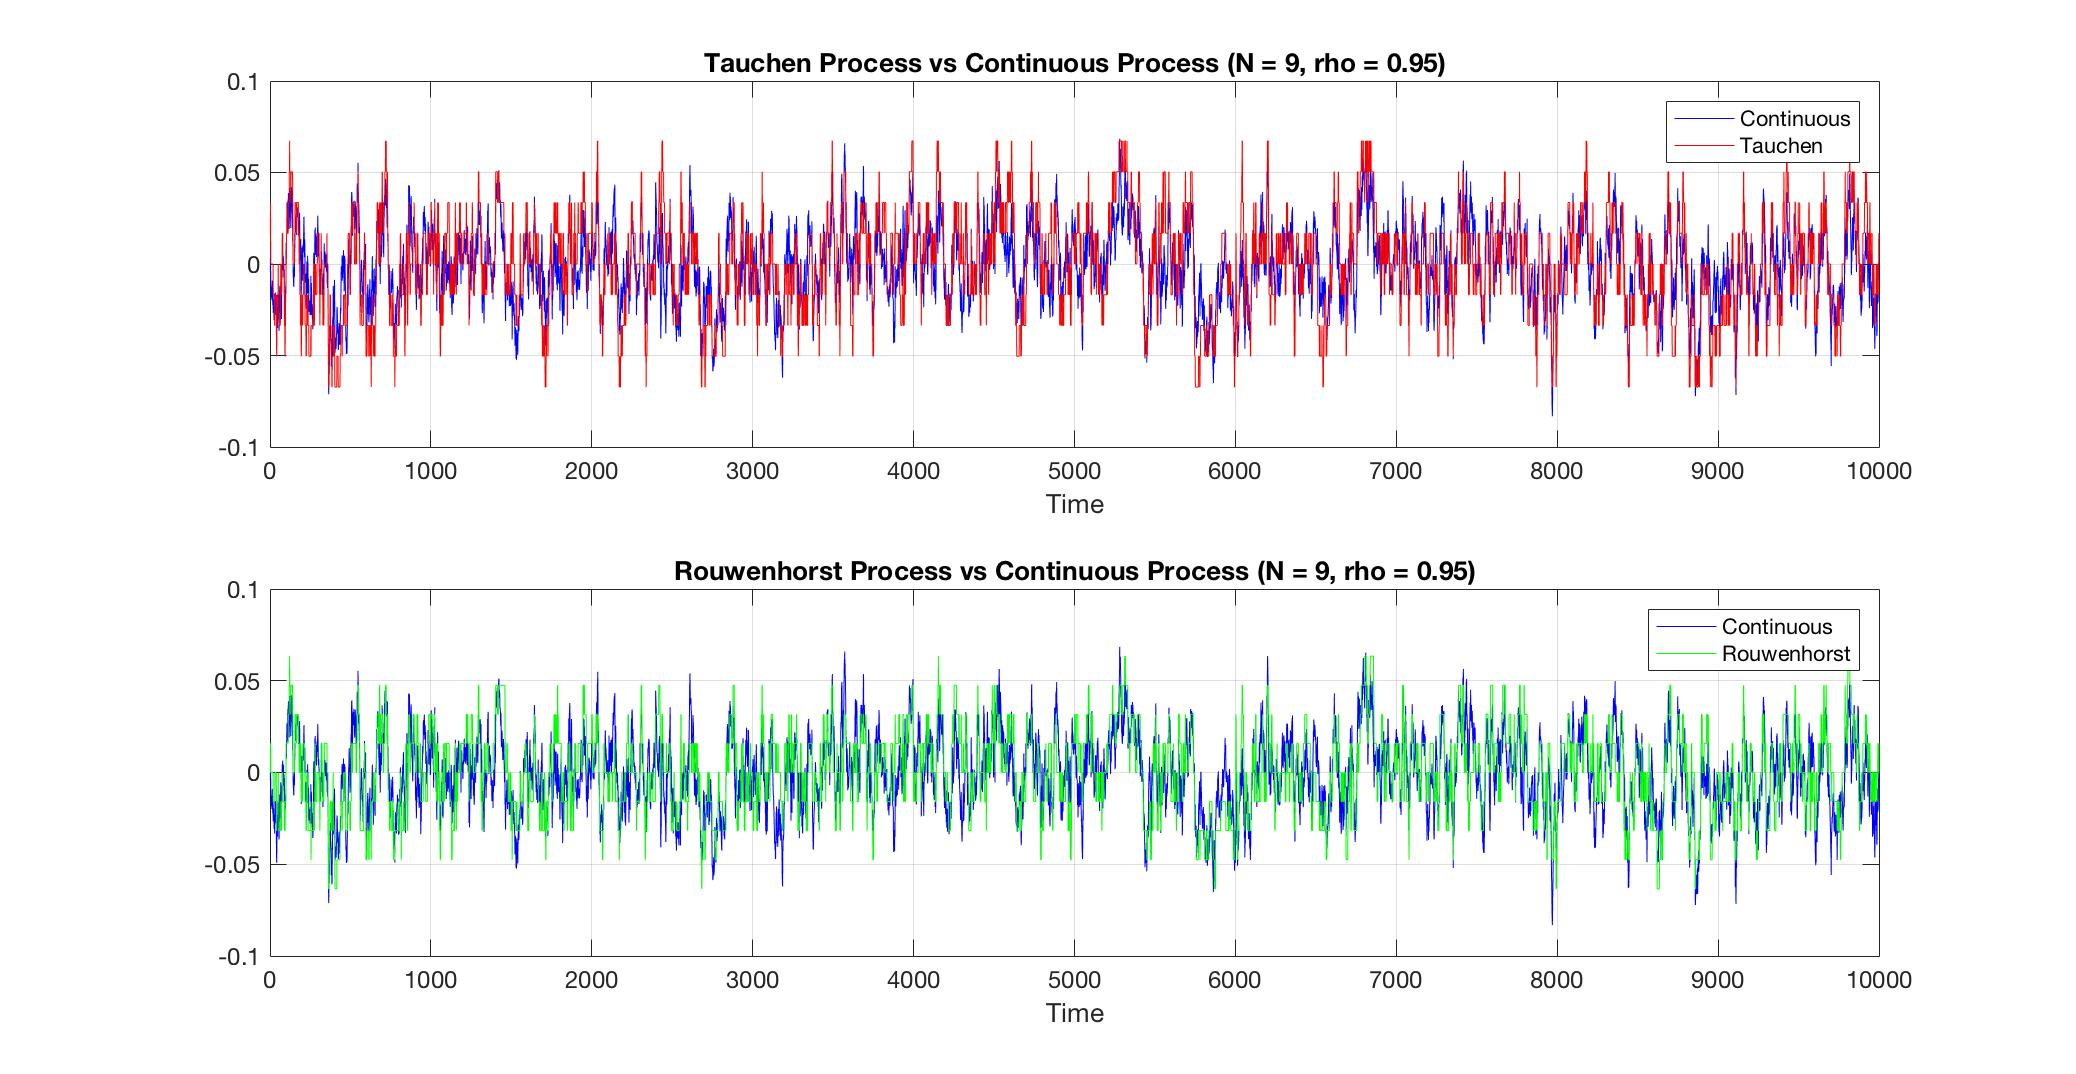
\includegraphics[scale = 0.22]{tauchen-vs-rou-n9.jpg}
	\caption{Simulação - $N = 9, \rho = 0.95$}
\end{figure*}

Computei também o Erro Quadrático Médio em cada caso e obtive quantidades comparáveis. No caso de Tauchen, o EQM foi de $2.5456\mathrm{e}{-04}$, enquanto o algoritmo de Rouwenhorst gerou um EQM de $2.2068\mathrm{e}{-04}$. Se adicionarmos mais pontos ao grid, teremos uma solução melhor. Passando para $N = 90$, a aderência ao processo azul aumenta consideravelmente.
\begin{figure}[h!]
	\centering
	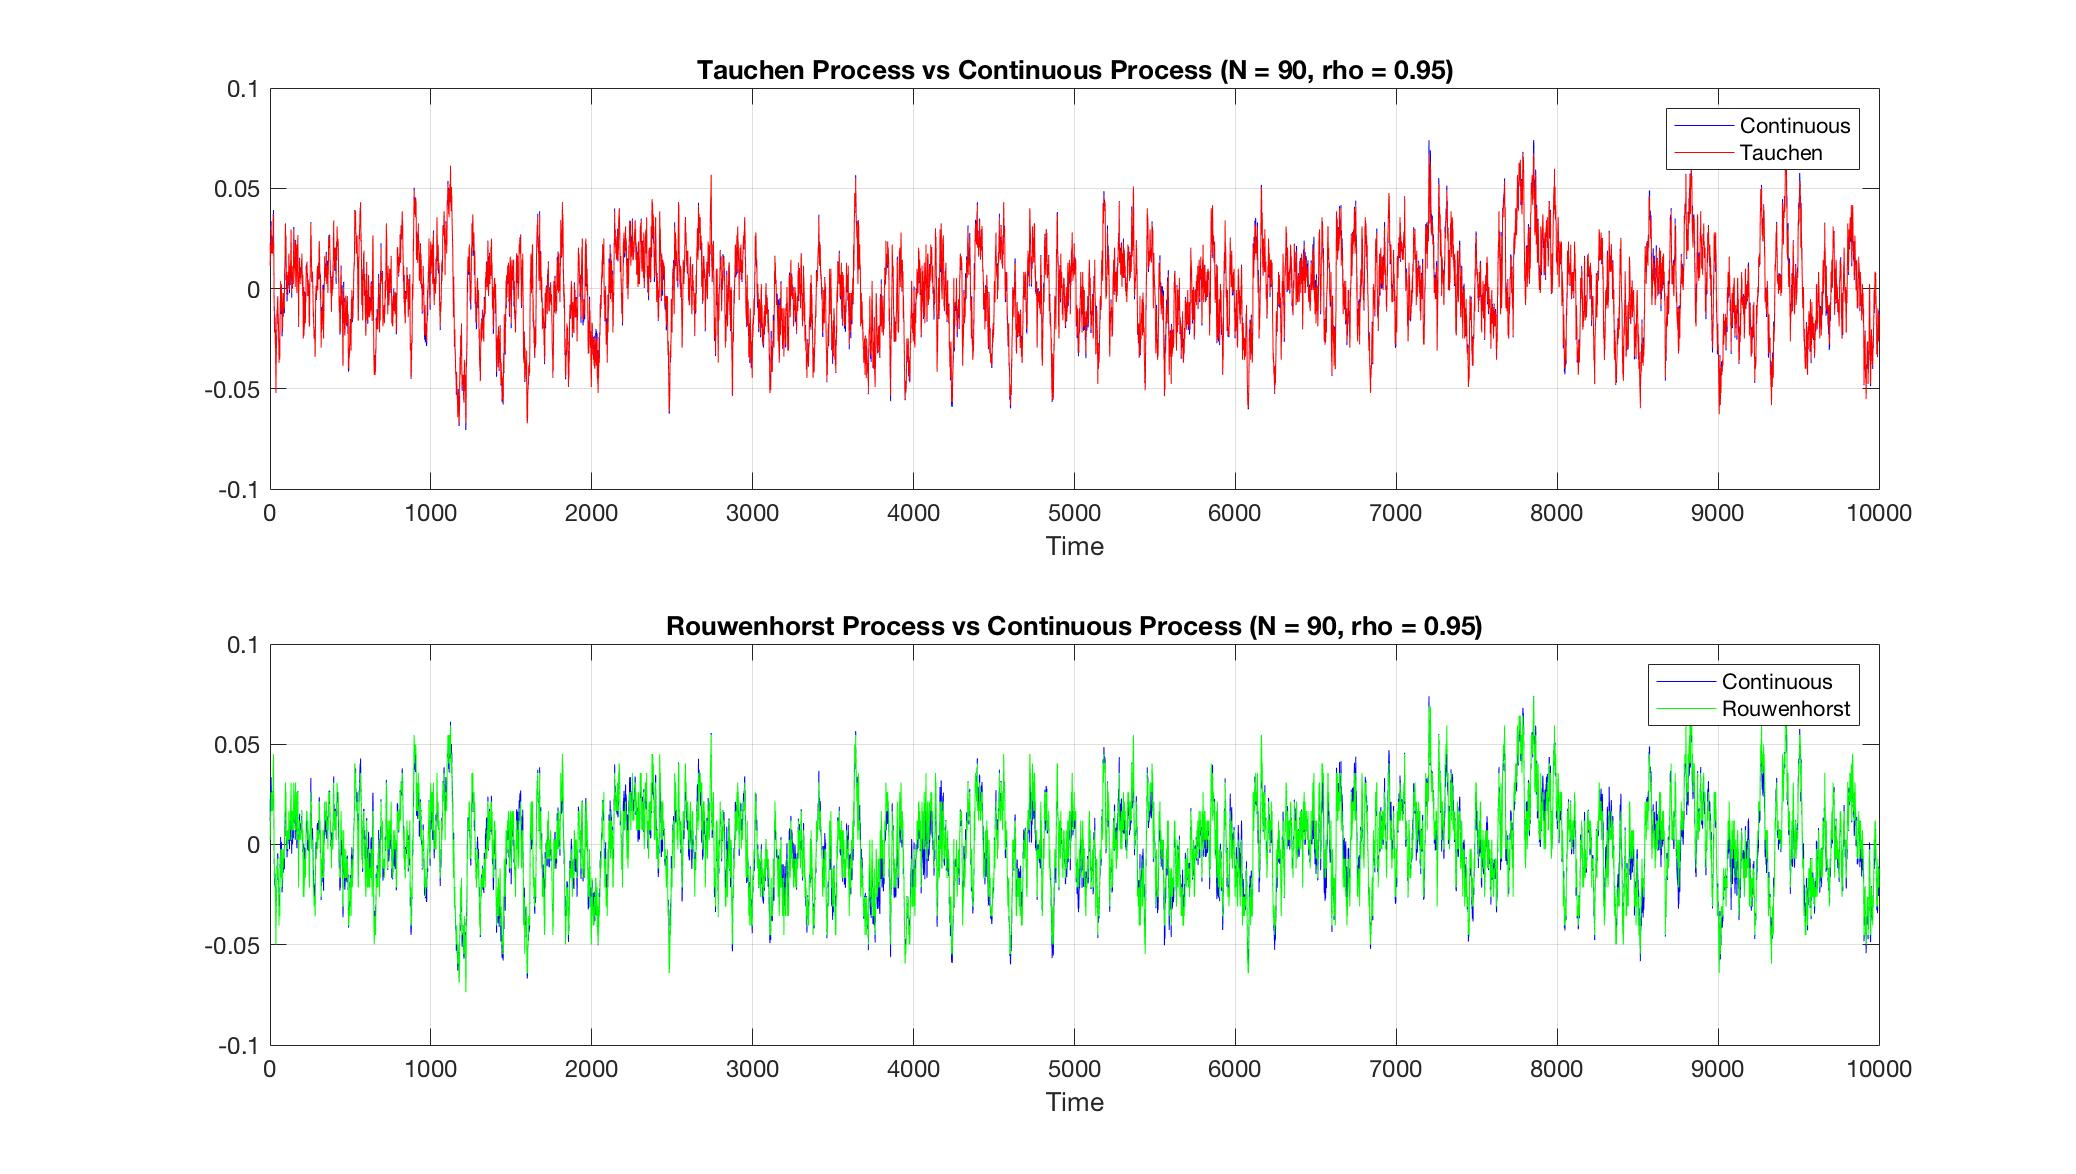
\includegraphics[scale = 0.22]{tauchen-vs-rou-n90}
	\caption{Simulação - $N = 90, \rho = 0.95$}
\end{figure}

Visualmente, as linhas vermelha e verde parecem cobrir melhor a linha azul, como era esperado. De fato, isto pode ser confirmado pelo cálculo do EQM: $1.9380\mathrm{e}{-06}$ no caso de Tauchen e $2.0595\mathrm{e}{-05}$ para Rouwenhorst. Nota-se que o EQM do método de Tauchen desta vez é de uma ordem de grandeza menor do que o de Rouwenhorst, indicando uma melhor performance.

O passo seguinte consistiu em validar as simulações estimando o parâmetro $\rho$ com base nos caminhos gerados pelos dois métodos. Com o método de Tauchen, e a calibração $N = 9$ e $\rho = 0.95$, pude estimar $\hat{\rho}_{Tauchen} = 0.9513$. Tendo por base a simulação feita através de Rouwenhorst, $\hat{\rho}_{Rouwenhorst} = 0.9492$.

Ao utilizar $N = 90$, os valores se tornaram  $\hat{\rho}_{Tauchen} = 0.9576$ e $\hat{\rho}_{Rouwenhorst} = 0.9482$. Ambos os métodos se saíram ligeiramente pior em termos de estimativas pontuais com um número maior de estados.

\section*{Calibração Alternativa: $\rho = 0.99$}
Tudo se mantém como antes a menos do aumento do valor de $\rho$ para 0.99. A próxima figura mostra a simulação do AR(1) contínuo, com variância maior do que o caso anterior, como era esperado:
\begin{figure*}[h!]
	\centering
	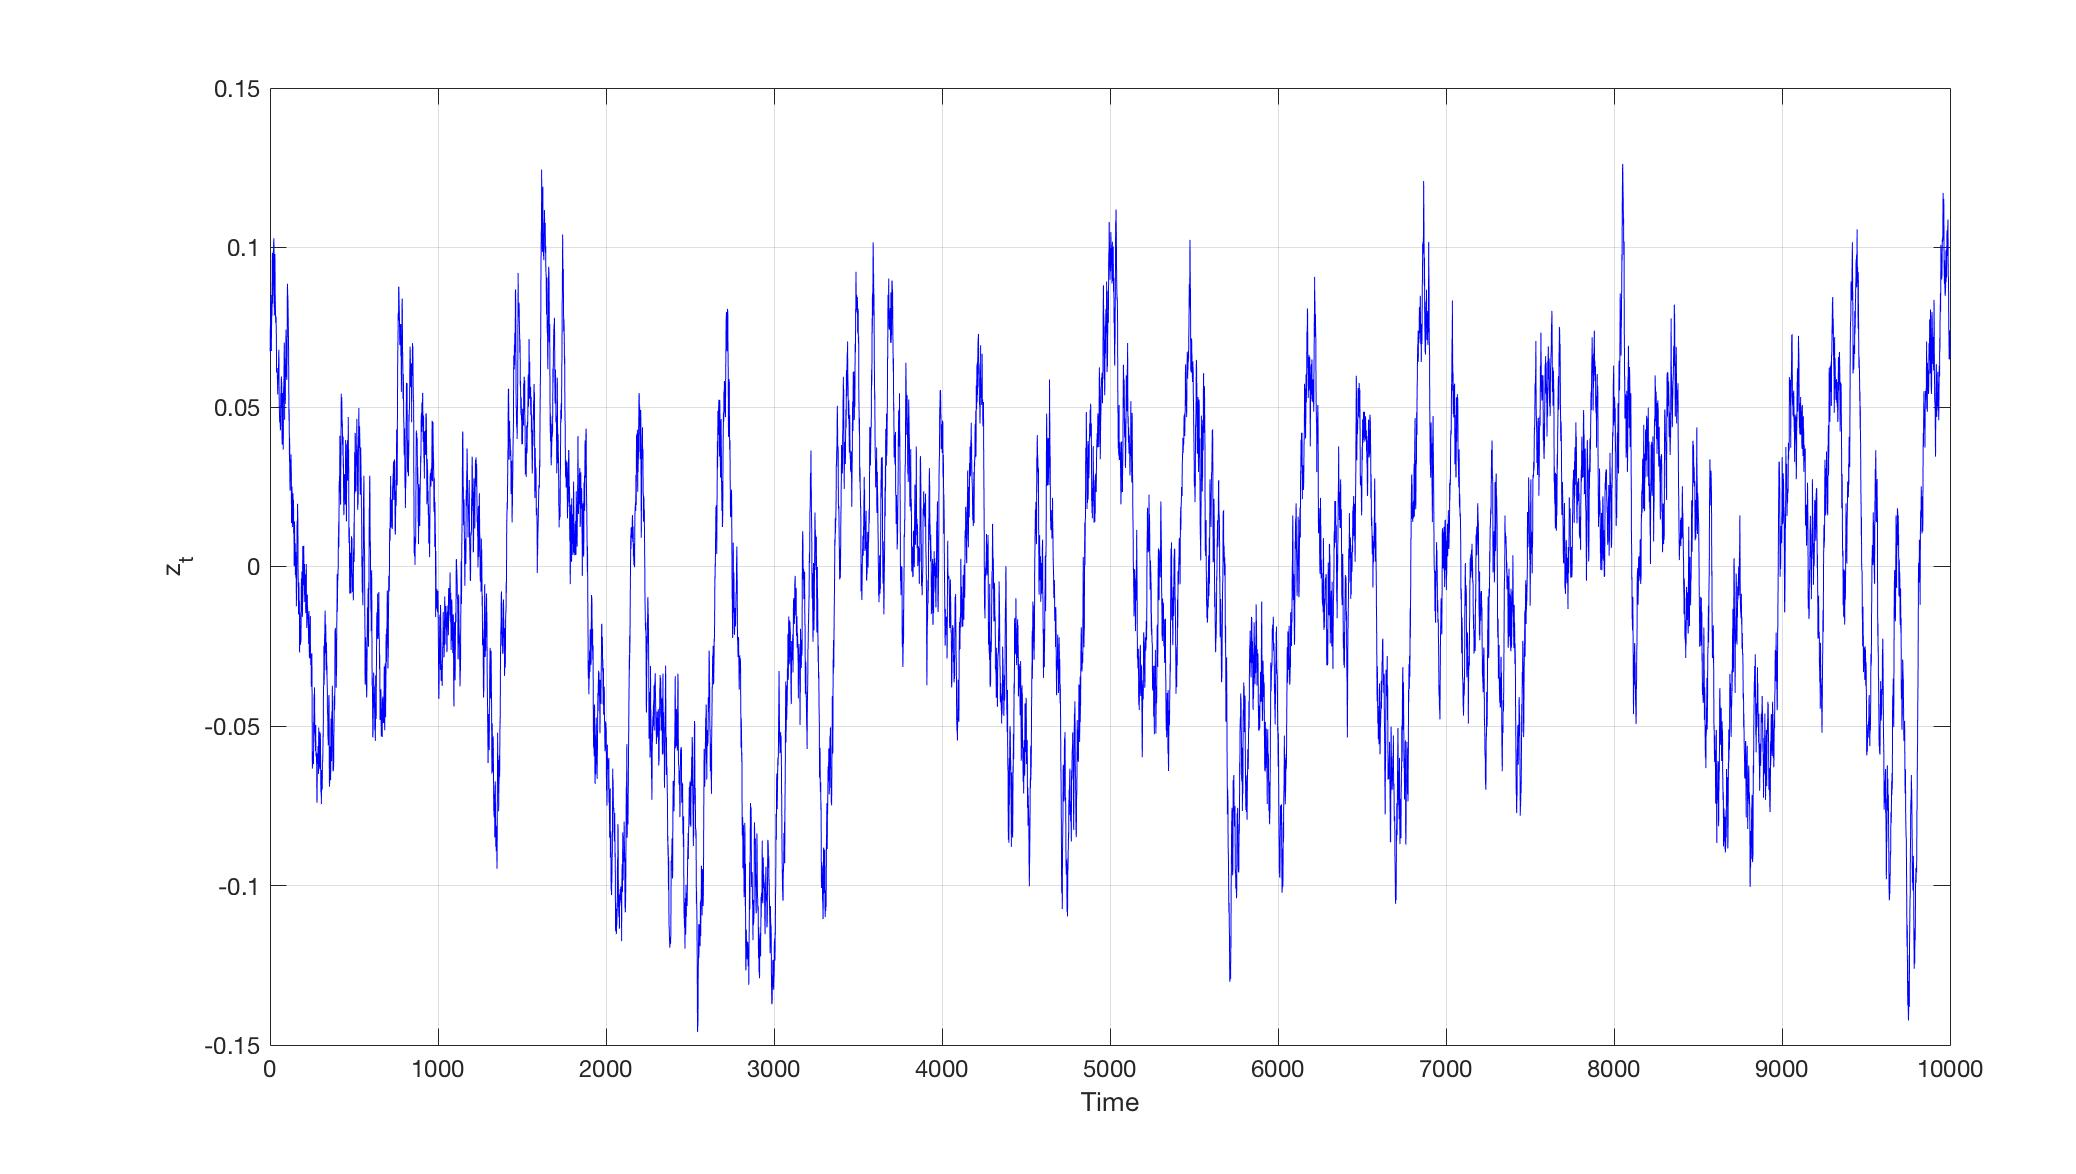
\includegraphics[scale=0.2]{cont_path_99.jpg}
	\caption{AR(1) Contínuo - $\rho = 0.99$}
\end{figure*}

Com respeito às simulações de Tauchen e Rouwenhorst, o primeiro método se saiu muito pior do que o segundo. Isto pode ser confirmado não só visualmente mas também através do EQM. Desta vez, os EQM's foram, respectivamente, $0.0074$ e $0.0030$. Nota-se que o EQM do método de Tauchen foi mais do que o dobro do EQM do método de Rouwenhorst. As estimativas de $\rho$ foram $\hat{\rho}_{Tauchen} = 0.9987$ e $\hat{\rho}_{Rouwenhorst} = 0.9892$.
\begin{figure*}[h!]
	\centering
	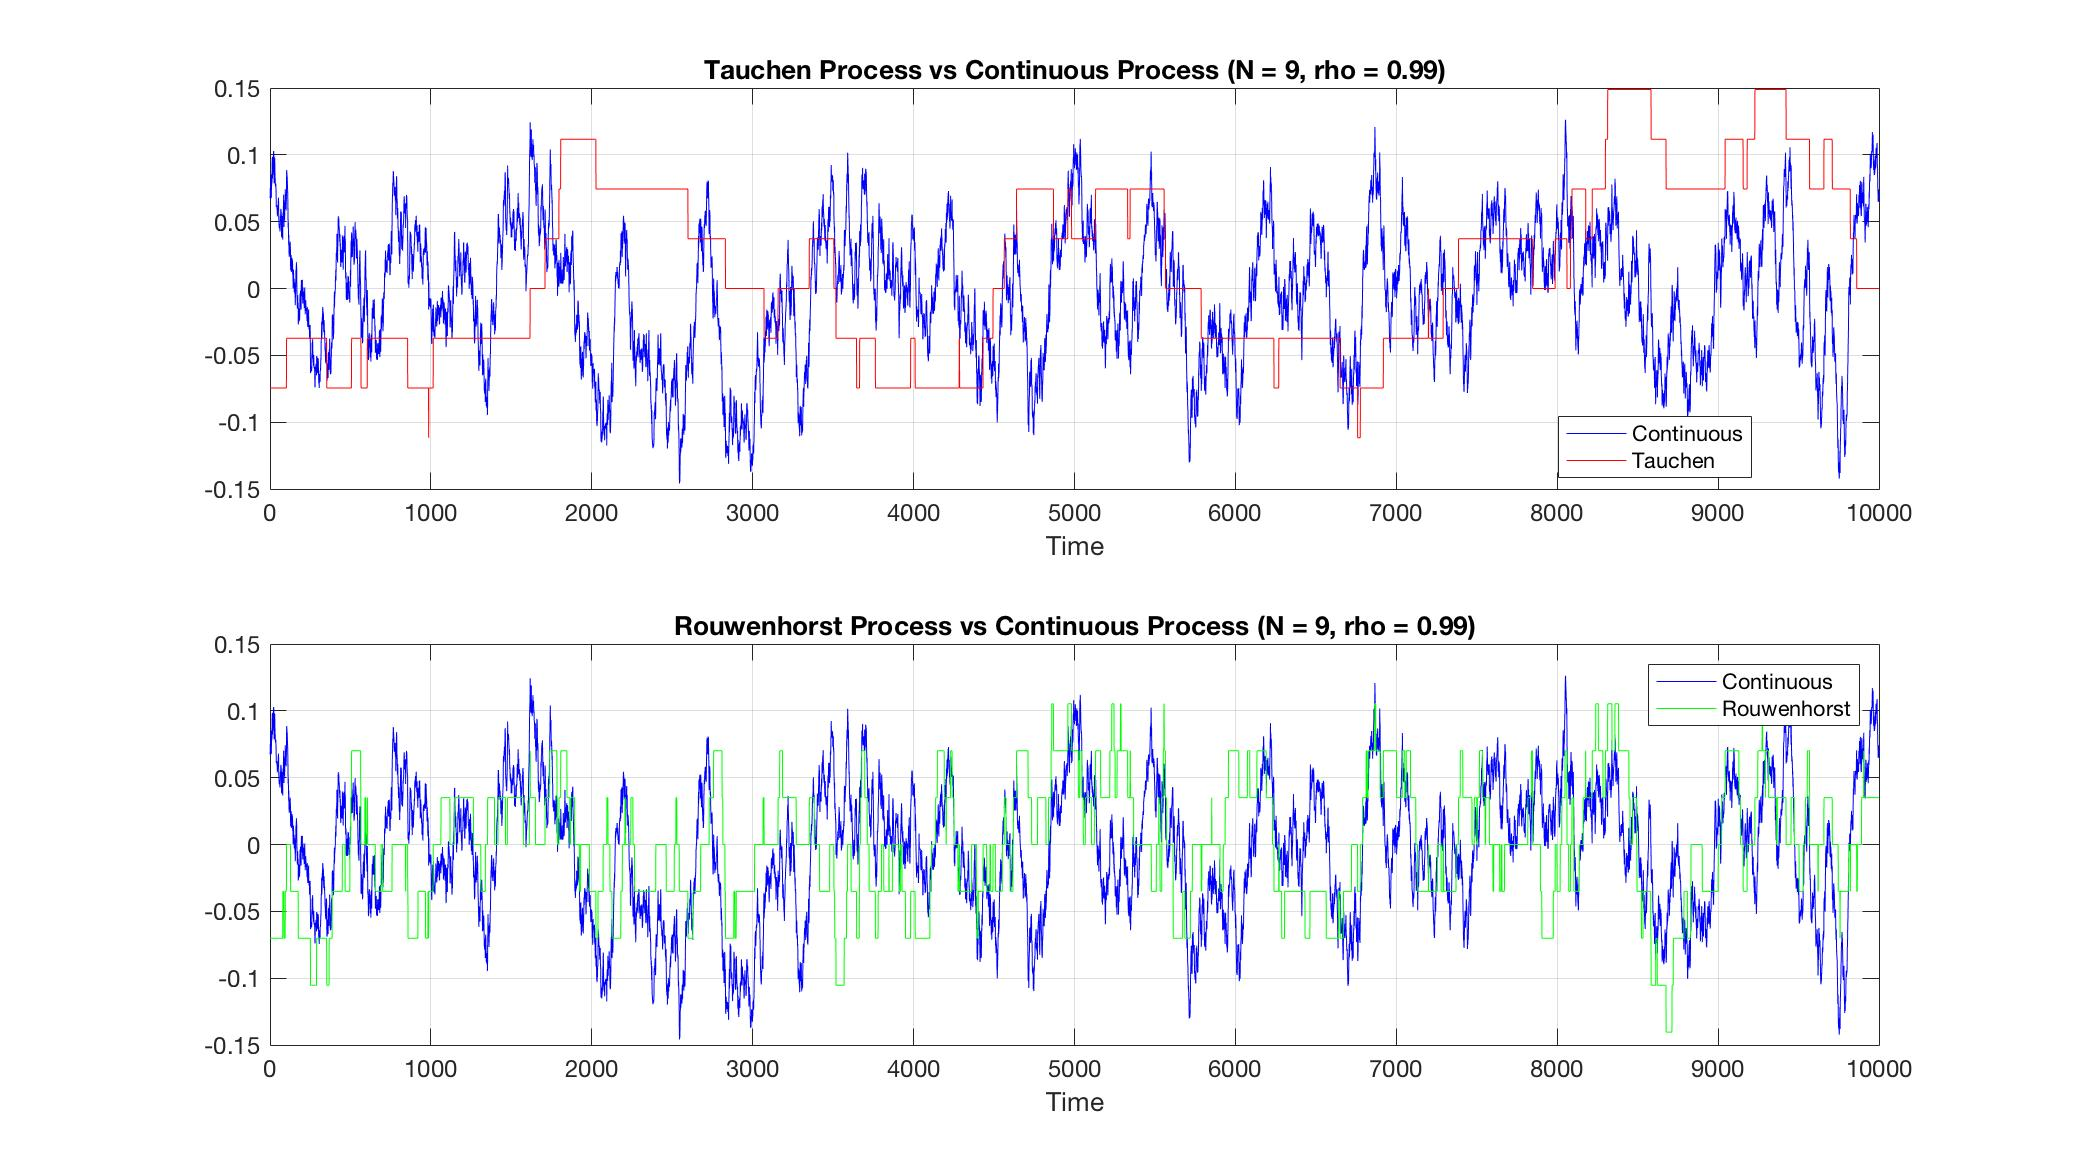
\includegraphics[scale = 0.26]{tauchen-vs-rou-n9-99}
	\caption{Simulação - $N = 9, \rho = 0.99$}
\end{figure*}

Se aumentarmos o número de pontos no grid para 90, assim como antes, temos o seguinte:
\begin{figure*}[h!]
	\centering
	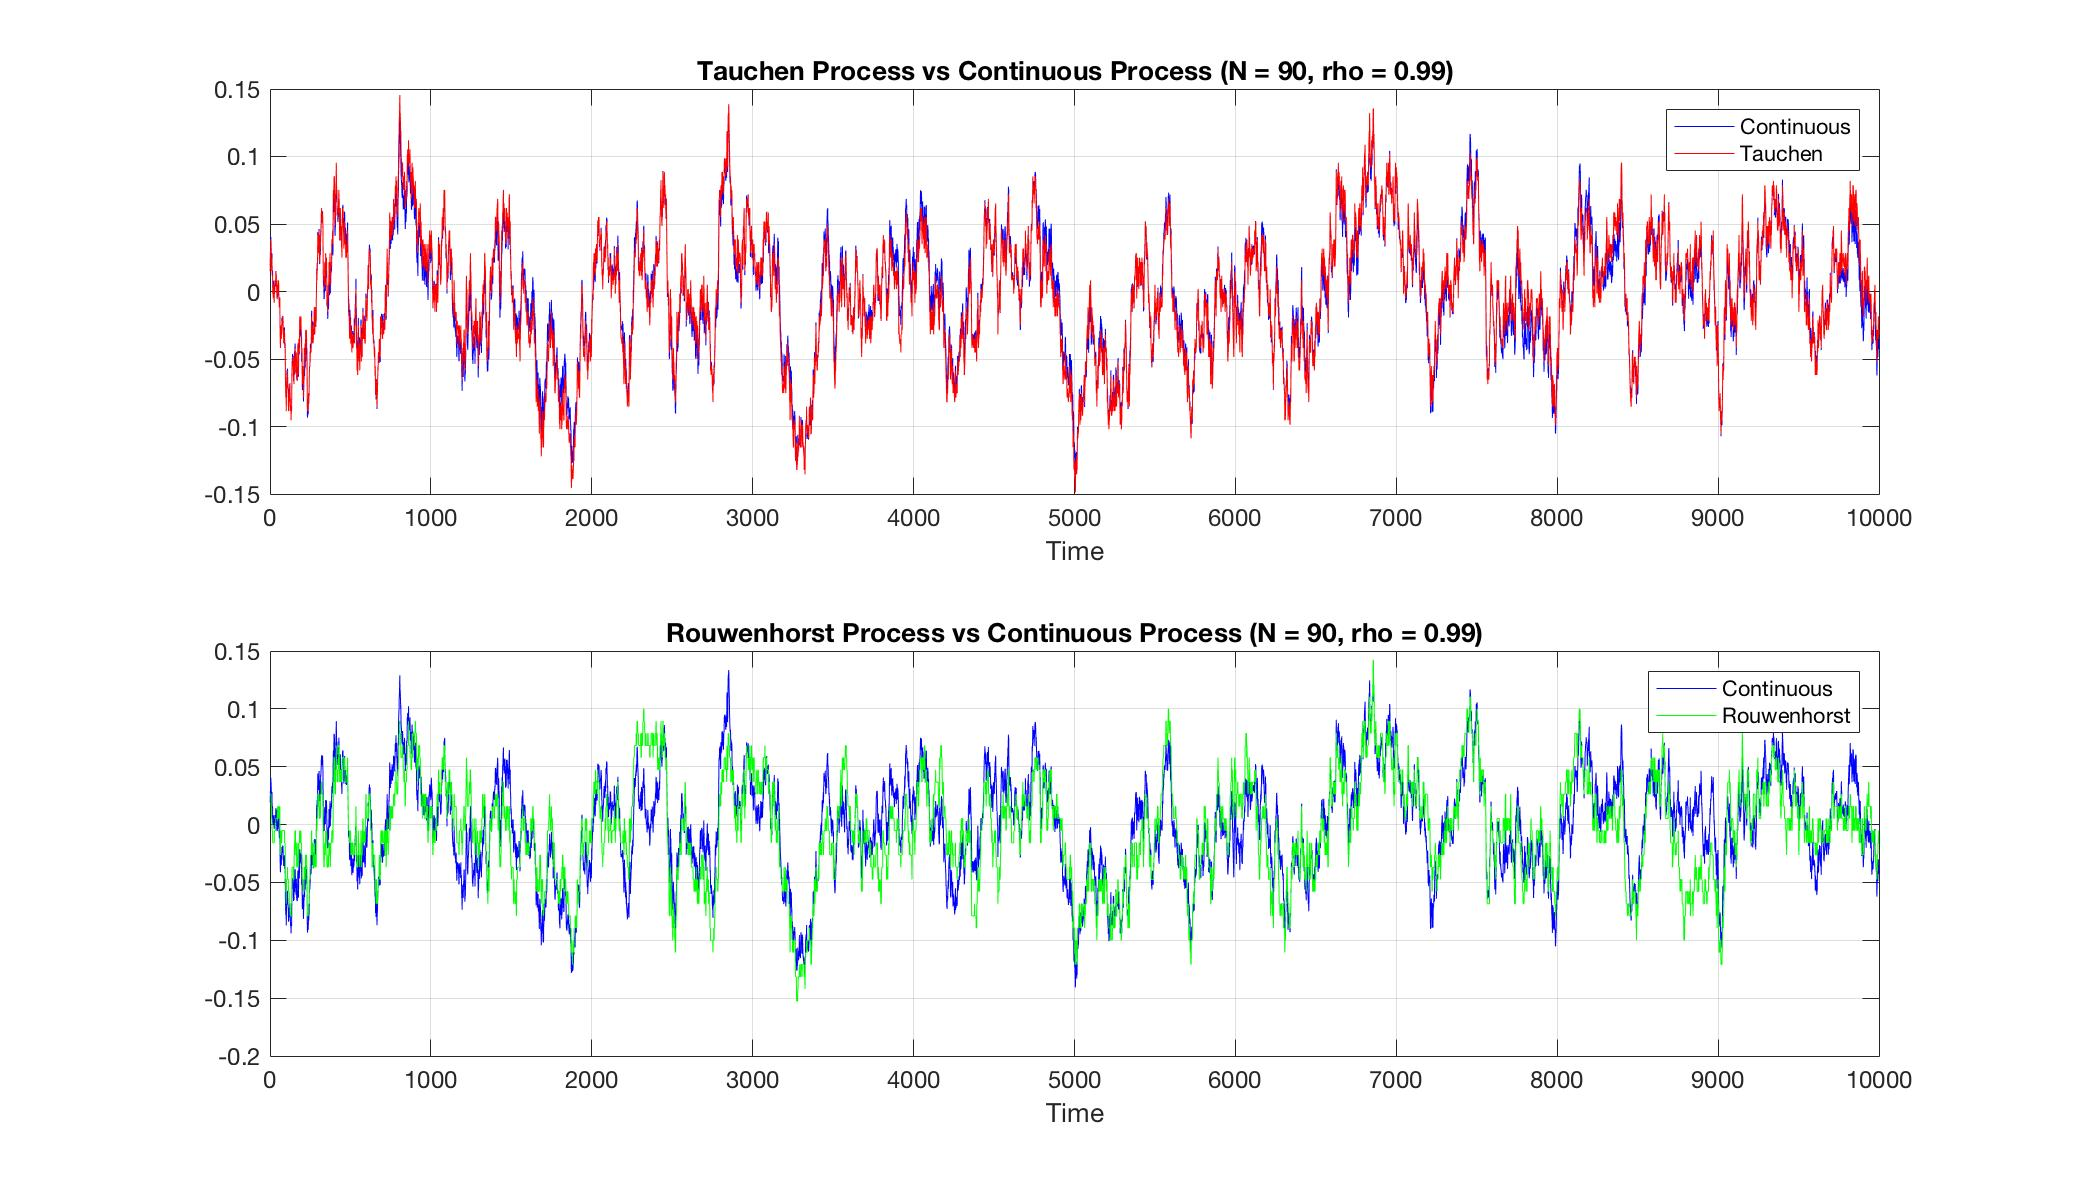
\includegraphics[scale = 0.26]{tauchen-vs-rou-n90-99}
\end{figure*}

O método de Tauchen melhorou muito seu desempenho. Inclusive, gerou EQM de $6.1956\mathrm{e}{-05}$, enquanto Rouwenhorst teve EQM de $5.9823\mathrm{e}{-04}$. As estimativas de $\rho$ foram $\hat{\rho}_{Tauchen} =  0.9881$ e $\hat{\rho}_{Rouwenhorst} = 0.9872$.

\end{document}